\section*{Related Work \& Background}

\subsection*{Static Scene Reconstruction}

Static scene reconstruction is the problem of reconstructing a 3D model from a set of 2D views.
Neural Radiance Fields (NeRFs)~\cite{mildenhall2020nerf} are a recent technique for reconstructing new views of a scene from new camera positions. To represent highly-detailed scenes, NeRFs model a scene as a continuous volume of varying density, which emits different colored light depending on the view direction. This is based on traditional volume rendering techniques:
\[ I(r) = \int_{t_n}^{t_f} T(t, r) \sigma(r(t)) c(r(t), r_d)dt, \]
where 
\[ T(t, r) = \exp(-\int_{t_n}^{t} \sigma(r(s))ds), \]
\noindent
where $I(r)$ is the illumination along camera ray $r(t) = r_o + r_d t$, $r_o, r_d$ are the ray origin and direction respectively, and $t$ is some positive distance along the ray. NeRFs are able to accurately reconstruct high-frequency features by recovering $\sigma$, the density at a given point, and $c$, the view-dependent color at a given point by modelling them as MLPs with an additional encoding scheme that can differentiate between extremely close points. NeRFs evaluate the above equations by performing ray-marching and computing $T(j,r) = \Sigma -\exp\sigma_i c_i$, by partitioning the ray into evenly spaced bins and sampling randomly from within each bin. There has been a plethora of work exploring NeRF and extensions which permit capturing more variance.

There have been a significant number of extensions to NeRF, including optimizations on the encoding for differentiating positions in space~\cite{tancik2020fourfeat}, better sampling approaches~\cite{barron2021mipnerf}, faster training~\cite{yu2021plenoxels}, and more~\cite{sitzmann2019siren}.

\subsection*{Dynamic NeRF Reconstruction}

Dynamic scene reconstruction is removing the assumption in static scene reconstruction that all views are under the same condition, such as the same lighting and that nothing has moved.
NeRFs were designed to only handle static scenes, and thus cannot accurately reconstruct scenes which contain movement, alternative lighting conditions, or other changes between frames.
In order to model dynamic scenes, there have been two diverging approaches.

One kind of approach directly models the transformation in the time domain, by learning a function $\sigma(x,t)=f(x\in\mathbb{R}^3, t\in[0,1])$, which include works such as HyperNeRF~\cite{park2021hypernerf}, NeRFies~\cite{park2021nerfies}, Space-Time Invariant Irradiance Fields~\cite{xian2021space}, and others~\cite{Wang_2021_CVPR,du2021nerflow}. By directly modelling the variation of the density, these methods are able to reconstruct large deformations in latent spaces and reconstruct a wide variety of transformations from a single radiance field. These often allow for fun transformations in some learned space between many similar scenes, which allow novelty warping and interpolation.

The other kind of approach models movement directly as translation. NeRFs are not able to move the objects inside the scene since we can only evaluate the NeRF at a given $x$. Instead we bend the rays, warping what is visible from a given view. This is essentially a perspective shift of a transformation of the space being rendered. Instead of moving an object that is seen by ray $r$, we warp ray $r$ such that it is sees the object. The equation for density is defined as $\sigma(x,t)=f(x+\Delta(x,t))$. This formulation enforces a coherent canonical representation, while directly modelling movement, and has been shown to be able to reconstruct both synthetic scenes with D-NeRF~\cite{pumarola2020dnerf} and real scenes in NR-NeRF~\cite{tretschk2021nonrigid}. There has also been work on recovering movements of entire NeRFs within a scene, such as in \cite{dynamicSceneGraphs}, but this work diverges from that approach as we are interested in reconstructing movement within a NeRF.

We note that a lot of prior work in this field not been peer-reviewed~\cite{pumarola2020dnerf,li2021neural,park2021nerfies,neural3dViewSynthesis}, but these works still have a significant impact, especially since the field moves quickly.

The pros of directly including time as a function in the MLP are that we are able to represent a much broader class of functions, in theory every frame may be fully distinct from the previous, but the movement formulation lends itself to smoothness between frames. Our approach falls into the movement category, as we are interested in accurately reconstructing smooth movement as opposed to generalizing over many classes of transformations.

\subsection*{Bezier Curves}

Bezier curves refer to a specific set of polynomials parametrized by a set of control points. They are most commonly used as cubic polynomials: $f(x) = ax^3 + bx^2 + cx + d$,
where $x$ is the variable we are interested in interpolating over. An example of a Bezier Spline is shown in Figure~\ref{fig:bezier_diagram}. The general formulation for
the Bezier basis functions is defined as $B^n(t) = \Sigma^n_{i=0}
{n \choose i} (1-t)^{n-i} t^i$ where $n$
is the degree of the Bezier polynomial. In order to give control of the Bezier curve, we
introduce "control points", which weigh different points along the curve differently:
$B^n(t) = \Sigma^n_{i=0} P_i {n \choose i} (1-t)^{n-i} t^i$, where $P_i\in\mathbb{R}^3$ for 3D
movement. For a more comprehensive guide on Bezier splines, we refer the reader to a more
\href{https://pomax.github.io/bezierinfo/index.html}{complete reference}~\cite{bezier_primer}.

\begin{figure}
    \centering
    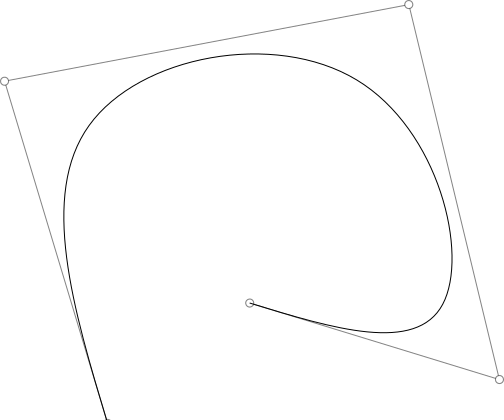
\includegraphics[width=0.2\textwidth]{bezier_curve.png}
    \caption{
        \textbf{Example of a Bezier Spline}.
        Bezier curves are a low-dimensional polynomial representation that allows for smooth interpolation between a few control points. We reconstruct control points to produce smooth movement and induce a prior on continuity. Bezier curves are common in both animation and drawing software.
    }
    \label{fig:bezier_diagram}
\end{figure}

